%!TEX root = ./report.tex
\section{Problem Analysis and Requirements}
In the following section we will analyse the presented problem, and discuss a set of requirements for a solution that is capable of editing a partial IFC model within a specific domain. This list should be thought of as a guideline for how this problem should ideally be approached, if the project results were to be replicated. The list is formed by theoretical knowledge, as well as experience gained through the course of the development of the solution.

\subsection{Problem Analysis}
\label{subsec:problem_analysis}
As described in Section \ref{sec:workflow}, the separation of the construction model and plumbing model causes it to be difficult to keep consistency between the two. In this project we will focus on how IfcFlowSegments (e.g. a pipe), IfcWallStandardCases (a regular wall) and an IFCOpeningElement (a hole in a regular wall) interact. Kaj Jørgensen mentions that a possible solution to the problem is to allow the building service engineer to create a message with precise information about required holes, or openings, for the pipes.(TODO insert reference) This message should then be handed to the construction engineer, such that he is able to verify that these are properly placed. A part of doing this is facilitating a transformation of IFC into a subset of the domain, where it is easy for the user to make changes to this subset, and reflect these changes back to the original IFC. As such, the primary goal of the solution is to enable the user to work on a subset of the IFC model involving pipes, openings, and walls. In Figure \ref{fig:ifcheirachy} a graphical representation of this subset is presented, excluding relational objects, such as IfcRelVoidsElement.

\begin{figure}[t]
    \centering
        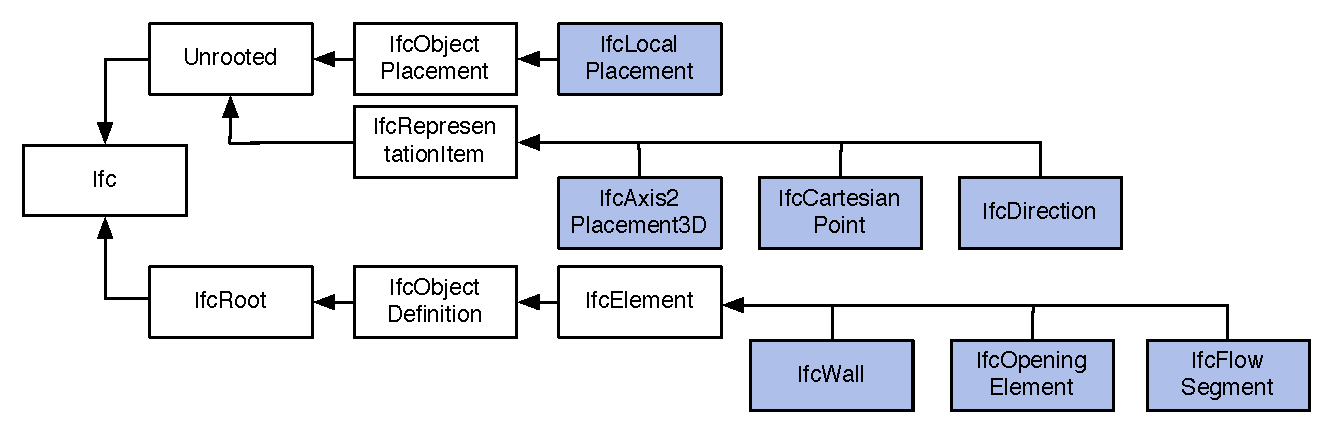
\includegraphics[width=120mm]{images/IfcHeirachy.pdf}
    \caption{A graphical representation of the subset used, excluding relational objects. The focus of the project are highlighted in blue.}
    \label{fig:ifcheirachy}
\end{figure}

\subsection{Requirements}
\label{subsec:requirements}
\paragraph{Working with a Partial Model}
With the aforementioned complexities and challenges of IFC in mind, a primary focus is to be able to extract a well-specified subset of the IFC. It is desirable to have an architecture that separates this concern from the rest of the workflow into one component, that extracts the partial model that we are interested in. Reversely, the problem of re-inserting this partial model should also be implemented as a modular workflow component. This allows for easy reuse of the module and makes the correctness of the extraction process verifiable.

Furthermore, a clear domain definition is needed to implement and verify the extraction process. To do this in a concise but generic way turns out not to be entirely trivial. An evolving standard for this kind of specification is Model View Definitions(MVD)\,\cite{nour08}, which is a precise but extensive standard that allows fine-grained IFC subset specification in XML. However, defining a partial model with MVD is in itself a complicated task and for purposes of designing a single experimental DSL with only a few IFC classes a more informal definition of the domain is preferable to simplify the development process\,\cite{mvd}.

\paragraph{Correct Meta Model}
When loading an IFC building instance from EXPRESS or ifcXML to Ecore it is vital for the solution that the IFC meta model is in fact correct. This point may at first seem trivial but in our experience a correct EMF meta model that reflects the actual IFC standard is difficult to obtain, especially one that comes with a proper serializer/deserialiser converting from either EXPRESS or ifcXML to the corresponding Ecore instance. The difficulty lies in the fact that across existing implementations, it is not at all consistent how models are treated, so one must be aware of any inconsistencies in the meta model\,\cite[pp. 4]{quteprints37725}. %FIXME: 

\paragraph{Valid Model Transformations}
An ideal solution would produce model transformations that are verifiable and correct. By verifiable, we refer to being able to trace that transformations actually occur in the way that we require. By correct, we primarily refer to not corrupting any model structure during a transformation, but also to not breaking any constraints in the domains. However, with the complexity of IFC in mind, we will relax the requirement to not breaking any constraints. As such, the ideal solution would show that making a valid model to model trasformation between and IFC partial model and a Pipes model is feasible.

\paragraph{A Simple DSL}
When all these technical features have been accounted for the solution still needs a simple DSL. Key to a non-experimental solution is that it displays a part of the complex source domain in a simple, manageable way. However, in this project, which is indeed very experimental, only the presence of a DSL will be listed as a desirable feature and not the syntax or usability of this. This being a feasibility study only the inclusion of a DSL as a proof of concept is relevant, as one could imagine that a future end product would indeed be visual instead of textual.

When implemented, a simple DSL will demonstrate that the partial model editing is feasible for any subdomain of IFC. In other words the implementation will show how a small but significant target domain, like the position of a pipe and a hole in a wall, can be managed separate from the main model. Therefore, to support extensibility and reusability, it should be build with wide-spread tools like EMF and Xtext.

\paragraph{Structural Editing}
A meaningful scope of what should be possible to do with the DSL, is the ability to edit existing values, say the position of a pipe, and more importantly, the ability to remove or add elements. The latter should be possible to resemble a real-world use case scenario, and the solution should be able to do this, of course, without corrupting the IFC instance.
\paragraph{}
This concludes the list of desirable features, but please note that it is only a core selection and that one could imagine many extensions to it. Some of these will be discussed in Section \ref{sec:future_work} as future work. 

